%
% RELATED NOTES (Richard)
%    PersonalJBArchive
%    PSnucleosynthesis/Branch-GalaxyAssemblyAndZDistribution 
%        */bhmetals   : paper.tex, paper-shorter.tex
\documentclass[nofootinbib,twocolumn,prd]{emulateapj}
\usepackage{hyperref}
\usepackage{amsmath}
\usepackage{graphicx}
\usepackage{color}
\usepackage{ifpdf}
\usepackage[normalem]{ulem}
%\usepackage{eps2pdf}

\newcommand\mc{{\cal M}_c{}}
\newcommand\editremark[1]{{\color{red}#1}}
\newcommand\jillianremark[1]{{\color{blue}#1}}
\newcommand\msun{M_\odot}
\newcommand\unit[1]{\text{#1}}
\newcommand\abbrvPSgrb{PSG}
\newcommand\abbrvPSellipticals{PSE}
\newcommand\abbrvKBLowZa{BD2010}
\newcommand\ForInternalReference[1]{}
\newcommand\modelDefault{A}
\newcommand\modelNiino{A'}
\newcommand\modelKW{D}
\newcommand\modelMannucci{D'}
\newcommand\modelKB{B}
\newcommand\modelPanter{C}
\newcommand\cqg{CQG}
\newcommand\E[1]{\left<#1\right>}
%\newcommand\aap{A\&A}
%\newcommand\apss{APSS}
%\newcommand\aaps{AAPS}
%% \newcommand\apjs{ApJ S}
%% \newcommand\aj{AJ}
%% \newcommand\apjl{ApJL}
%% \newcommand\mnras{MNRAS}
%% \newcommand\pasp{PASP}
%% \newcommand\pasj{PASJ}
%% \newcommand\araa{ARAA}
%% \newcommand\physrep{Phys. Rep.}


\begin{document}
\title{Details matter: Similar host galaxies can harbor different merging compact binary populations} 
\author{R.\ O'Shaughnessy}
\affiliation{Center for Computational Relativity and Gravitation, Rochester Institute of Technology, Rochester, NY 14623, USA}
\email{oshaughn@mail.rit.edu}
\author{ J. Bellovary}
\affiliation{Department of Physics, Queensborough Community College, Bayside, NY 11364}
\email{jbellovary@qcc.cuny.edu}
\begin{abstract}
% POINT:
% - existence proof by example .. not an attempt to solve the general problem we raise
Galaxy formation
simulations can reproduce present-day galaxies with notably different assembly and star formation histories.  
Recent simulations of compact binary evolution suggest the compact object merger rate depends
sensitively on the progenitor's metallicity, to the extent that rare low-metallicity star formation during galaxy
assembly can produce more detected compact binaries than typical star formation.   
Using detailed simulations of galaxy and chemical evolution, we demonstrate by example that galaxies with similar present-day appearance can host distinctly different
compact binary populations.
We discuss the implications for transient multimessenger astronomy with compact binary sources. \jillianremark{Add quantifiable stuff when we have it.}
%% Present and future observations of  merging compact binaries can provide valuable constraints on their birthrate
%%  and formation scenarios.  However, recent binary evolution simulations suggest the compact binary merger rate depends
%% sensitively on the progentior's metallicity, to the extent that rare low-metallicity star formation during galaxy
%% assembly can produce more detected compact binaries than typical star formation.    Additionally, galaxy formation
%% simulations can reproduce present-day galaxies with notably different assembly and star formation histories, with
%% corresponding different present-day merger rates.  
%% % POINT 0: Gasoline + popsyn: real work was done
%% Using existing simulations of the assembly,  chemical evolution, and compact-object formation rate of a single halo
%% Milky Way-like galaxy with Gasoline, we construct present-day compact binary merger rates using a simple semianalytic
%% compact binary formation model ($dP/dt \propto Z^\alpha/t $) motivated by detailed calculations in the literature. 
%% % POINT 1: Observations
%% %   - difficult to reconstruct f
%% %   - local particle far away
%% As expected, we show the present-day galactic state can be only weakly correlated with the dominant compact binary
%% fomation rate: the galaxy could form in several ways, including epochs of low-metallicity star formation through major
%% mergers; and present-day mergers rarely occur near gas with their progenitor metallicity, even when not kicked.  
%% %  - but the galaxy 
%% By contrast,  detailed studies which reconstruct the galaxy's star formation history and metallicity evolution could,
%% when stacked, pinpoint the dominant formation process \editremark{need more than handwaving}.
% POINT 2: Revised merger rates
%% Averaging over the cosmological star formation history and galaxy mass-metallicity relation, we demonstrate low
%% metallicity star formation can produce much of the detected population of short GRBs and nearly all gravitatational-wave
%% sources. 
%% % POINT 3: Challenge for observations
%% Therefore,  though a potentially large fraction of binaries formed from low-metallicity gas,  their birth metallicity
%% cannot be identified directly, even with spatially resolved observations. 
%% %
%% We discuss the extent to which observations can distinguish between different scenarios for  low-metallicity compact
%% binary formation.
%
%\textbf{say something using GRBs in paragraph; perhaps mention relative bias in $p(M_g|GRB)$ relative to prior?}
%% \textbf{say something about different SFR histories making present galaxies -- can do more if we can distinguish history
%% of the galaxy}

\end{abstract}

%% absolutely critical vs optional
%
% critical
%  -write paper as is, minmal
% optional
%  - add dwarfs. They are important
%  - add ems counterparts. They are important
%  - discussion of multimessenger astro

\maketitle

\editremark{We will be very careful to specify how SFR and metallicity are measured, backtracking}

Add me: \cite{Kirby13}
Add me but note conflict \cite{Somerville15}, etc

Add me: \citet{Madau14}

Add me: Hopkins et al  \cite{2016arXiv160508783L} (in context of similar model, building off my prior work)

\section{Introduction}
% POINT: LIGO soon will detect compact binary mergers....
%     ... and possibly EM counter part too
%     ... which will enable new physics
Gravitational waves have been detected from  coalescing  black hole binaries \citep{DetectionPaper,LIGO-O1-BBH}. 
Over the next few years, ground-based gravitational wave detectors like LIGO 
and Virgo  should detect the gravitational
wave signal from many more similar merging compact binaries \citep{LIGO-O1-BBH,RatesPaper,gwastro-EventPopsynPaper-2016}, as well as  binary  neutron stars and black hole-neutron star binaries \citep{LIGO-Inspiral-Rates,popsyn-LowMetallicityImpact2c-StarTrackRevised-2014}.
%
The host galaxies of gravitational wave sources will be identified, either directly or statistically.  
On the one hand, addition to the strong gravitational wave signal, mergers of neutron stars are expected to  frequently be accompanied by detectable
electromagnetic radiation  via a number of  mechanisms, including a strong but tightly beamed
ultrarelativistic jet and weakly-beamed but more isotropic thermal radiation from an expanding hot shell
\citep[see,e.g.,][and references therein]{2013PhRvL.111r1101C,short-grb-GWCoincidenceEM-MetzgerBerger2011}.  
% People we can't afford the space to cite, alas:
%    - 2015arXiv150101986H   -
%    - 2013MNRAS.430.2121P - Rosswog recent
%    - Shibata group/Koutarou
In addition to providing a wealth of information about the merger event itself, a multimessenger detection will pin down
the sky position and therefore approximate birthplace of each merging binary.    
%
On the other hand, gravitational wave detectors can perform high-precision sky and volumetric localization \cite{2016LRR....19....1A,2016arXiv160307333S}.  As GW detector
networks increase in sensitivity, these localizations will allow statistical and, eventually, unique identification of
host galaxies directly, even without associated electromagnetic emission.
%
As with supernovae and  GRBs, these host galaxy associations   are expected to tightly constrain models for compact binary
formation; see, for comparison,  \citet{2011MNRAS.412.1508M}, \citet{long-grb-GuettaPiran2007},
\citet{2014ARAA..52...43B}, and references therein. %2010ApJ...722.1879M,2010MNRAS.407.1314M}.     
%

% POINT: Huge detail possible
The host galaxies of distant short GRBs have already been extensively investigated, with the associations being used to
draw preliminary conclusions about their progenitors  \cite{2014ARAA..52...43B}.   
%Of necessity, these analyses  on bulk correlations, often stacked to increase significance across multiple sources
%\editremark{clean up/don't piss off   Edo}.  
Unlike GRBs, detected gravitational wave sources will be limited by the range of LIGO to the local universe; for
example,  binary neutron star sources should be closer than $400\unit{Mpc}$.  Due to their proximity, each host galaxy
can be explored at great depth and detail via  position-resolved spectroscopy, enabling detailed position-resolved star-formation
and chemical evolution histories \editremark{citation: need better ones} \citep[see,e.g.][]{2009MNRAS.396..462K,2014MNRAS.444..336C}. \jillianremark{Do you want citations of GRB host observations or just general galaxy stuff?}
% POINT: But is it useful?
In this work, we demonstrate by concrete example that detailed analysis of individual galaxies can be essential to
investigate key physical questions about the origin of compact binary mergers. 



This paper is organized as follows. 
In \S \ref{sec:sims}, we describe detailed hydrodynamical simulations of  two galaxies.  Though these two
galaxies are at  present similar to the Milky Way, we
show that their star formation and chemical evolution history have subtle but important differences due to their
distinctive merger histories.   To demonstrate
these differences have a significant practical impact,  in \S \ref{sec:model}, we introduce a simple,
metallicity-dependent  phenomenological model to calculate the present-day rate and mass distribution of compact binary
mergers from  a galaxy's known history.   In \S \ref{sec:results:BBH}, we use this model to demonstrate the binary black hole coalescence rate
depends sensitively on the galaxy's assembly history, in a manner which is far from apparent from its present-day
properties.  
In \S \ref{sec:results} we show that while these two galaxy formation models should produce comparable detectable binary neutron star
populations, these two scenarios could produce dramatically different populations of electromagnetically detectable
merging black hole-neutron star binaries. 
%


%% %   - Delay  time only: 
%% For example, the lag between transients' redshift distribution and the past star formation rate has shown long GRBs are
%% associated with short-lived progenitors (see, e.g., \cite{long-grb-GuettaPiran2007} \cite{grb-long-Virgili2011-TryingEverything} and
%% references therein) and that SNIa merge long after their formation
%% \citep{sn1a-DelayTimeDistribution-Cosmological-Graur2011}. \editremark{other cites}
%% % * \cite{YoungLongGRBHostPredictions2007,FryerGRBProgenitorConstraints2007} : Long bursts.
%% By contrast, short GRBs noticably lag cosmological star formation  \editremark{Berger; }\cite{2007ApJ...665.1220Z,Nakar} 




\section{Cosmological simulations produce two distinct Milky-Way-like galaxies}
\label{sec:sims}

\subsection{Simulating galaxy evolution}
To thoroughly study the significance of low metallicity star
formation, we examine cosmological smoothed particle hydrodynamics
(SPH) $N$-body simulations of Milky Way-like galaxies with GASOLINE
\citep{Stadel01,Wadsley04}.  These simulations allow us to analyze both
spatially and temporally resolved star formation, and determine not
only the metallicity history of compact object progenitors, but also
their dynamical evolution.  
%maybe move the below section to later and/or consolidate
One simulation we report here, $h258$,
involves the formation of a Milky Way-like disk galaxy whose
progenitors undergo major mergers at $z = 2$ and $z = 0.8$.  This
simulation has been previously discussed by
\citet{Governato09,Bellovary10,Bellovary11,Brooks11}; however we have
re-run the simulation at a factor of two higher in spatial resolution
and additionally included new physics including a prescription for
cooling by molecular hydrogen \citet{Christensen12}.

We selected our simulated region of interest from a 50 Mpc volume of
uniform resolution, and resampled the region at very high
resolution using the volume renormalization technique \citep{Katz93}.
This technique allows us to follow the detailed physical processes
involved in galaxy evolution in our selected region while still
including large-scale torques from cosmic structure.  We use
WMAP3 cosmology \citep{WMAP3} and model the ionizing UV background
with the prescription from \citet{Haardt96}.  Stars form
probabilistically from gas particles which meet density ($n_{min} =
10$ amu cm$^{-3}$) and temperature ($T_{max} = 10^4$ K) thresholds. If a gas
particle meets these criteria, it has a likelihood of forming a star
particle (representing a simple stellar population with a Kroupa IMF
\citep{Kroupa}) which is given by

\begin{equation}
p = \frac{m_{\rm gas}}{m_{\rm star}} (1 - e^{c^*\rm X_{\rm H_2} \Delta t/t_{\rm form}})
\end{equation}

\noindent
where the star formation efficiency parameter $c^*$ is set to 0.1 such
that our galaxies match the observed Kennicutt-Schmidt law
\citep{Kennicutt89};  X$_{\rm H_2}$ is the molecular hydrogen fraction of the gas particle; $m_{star}$ and $m_{gas}$ are the star and gas
particle masses;\footnote{In our high-resolution simulations \textbf{ROS-check!}\jillianremark{this number is correct, is that what you want to check? - JMB}, each gas particle starts with a mass
  $m_{gas,0}=26,676 M_\odot$, gaining mass from feedback and losing it to star formation.  Each star particle, when
  formed, has $1/3$ of the progenitor mass of the forming gas particle.  See \cite{Christensen10} for a discussion
of resolution issues in these SPH simulations.} $t_{form}$ is the dynamical time for the gas
particle; and $\Delta t$ is the time between star formation episodes,
which we set to 1 Myr.  We model supernova feedback using the
blastwave formalism described in \citet{McKee77} and implemented in
our simulations as in \citet{Stinson06}.  Each supernova releases
$E_{SN} = 10^{51}$ erg into the surrounding gas with a radius
determined by the blastwave equations.  These particles are not
allowed to cool for the duration of the blastwave, mimicking the
snowplow phase of a supernova explosion.  Previous works have found
that this set of parameters results in realistic galaxies which obey a
number of observed relations such as the mass-metallicity relation
\citep{Brooks07}, the Tully-Fisher relation \citep{Governato09}, and
the size-luminosity relation \citep{Brooks11}, as well as reproduce
the detailed characteristics of bulgeless dwarf galaxies
\citep{Governato10} and the Milky Way \citep{Guedes11}.


Also included in our simulations is a scheme for turbulent metal
diffusion \citep{Shen10}.  Metals are created in supernova explosions
and deposited directly to the gas within the blast radius.  Stellar
masses are converted to ages as described by \citet{Raiteri96}, and
stars more massive than 8 M$_\odot$ are able to undergo a Type II
supernova.  We follow metal enrichment from both Type II and Type 1a
supernova, with metal yields derived from \citet{Weaver93} and
\citet{Thielemann86} respectively.  From this point onwards metals
diffuse through the surrounding gas, according to 
\begin{equation}
\frac{dZ}{dt}|_{diff} = \nabla (D \nabla {Z}) \\
\end{equation}
%
where the diffusion parameter $D$ is given by
%
\begin{equation}
D = C_{diff} |S_{ij}| h
\end{equation}
%
and $h$ is the SPH smoothing length, $S_{ij}$ is the trace-free shear
tensor, and $C_{diff}$ is a dimensionless constant which we set to a conservative value of 0.03.  

%Sijing finds that C = 0.05 makes for a good comparison to clusters, and that C = 0.05 - 0.1 is expected from turbulence theory.

We identify individual galaxies using the halo finder $AHF$
\citep{Gill04,Knollmann09}, which identifies halos based on an
overdensity criterion for a flat universe \citep{Gross97}.  For this
work, we are focusing on the primary (i.e. most massive) galaxy at any
given redshift, which serves as the progenitor to our $z = 0$ Milky
Way-like galaxy.



\subsection{Two Milky-Way-like galaxies with distinct histories }

{\bf Richard go ahead and edit this however is needed.}  The evolution
of a galaxy, in terms of its stellar mass and metallicity evolution,
depends strongly on its interaction history.  Galaxies which appear
similar at the present day may have had drastically different
histories, which may result in differences in compact object merger
rates.  To investigate whether galaxy history affects the GRB event
rate, we have chosen two simulations which are extremely similar at $z
= 0$ but differ strongly in their merger histories.

The simulation h277 (Boring Galaxy) is a Milky Way analog with a
quiescent merger history.  It experiences its last major merger at $z
= 3$, after which a small number of minor interactions permeate its
life.  This simulation has been shown to emulate several Milky Way
properties, including stellar dynamics
\citep{Loebman12,Loebman14,Kassin14}, baryon fraction
\citep{Munshi13}, halo properties \citep{Zolotov09,Zolotov10}, and
disk properties \citep{Brooks11}.  It has a virial mass of $M_{vir} =
6.79 \times 10^{11} \msun$, stellar mass $M_* = 4.24 \times 10^{10}
\msun$, and maximum circular velocity $v_{circ} = 235$ km s$^{-1}$.

  The simulation h258 (Exciting Galaxy), on the other hand, has a much
  more active merger history.  At $z = 1$ there is a 1:1 merger event;
  a gas disk rapidly reforms following the collision (see
  \citet{Governato09}), resulting in a massive disk galaxy at $z = 0$
  which looks remarkably similar to the Milky Way and to the other
  simulation, h277.  Prior to the $z = 1$ merger, each of the two
  progenitor galaxies actually experiences its own additional major
  merger events around $z = 2$.  The combination of
  the series of major mergers, plus a number of minor interactions and
  flybys, gives a stark contrast to the relatively quiescent history
  of h277.  At $z = 0$, h258 has a virial mass of $M_{vir} = 7.74
  \times 10^{11} \msun$, stellar mass $M_* = 4.46 \times 10^{10}
  \msun$, and maximum circular velocity $v_{circ} = 242$ km s$^{-1}$.  \editremark{Might we want to show the images of these galaxies?}


  Due to the differences in merger histories, the metallicity
  evolution of h258 and h277 also differ at early times.  Figure
  \ref{fig:TwoGalaxies} shows the history of the mean metallicity of
  recently formed stars vs time (thick solid lines), where we define
  recent as within the past 50 Myr.  The shaded regions correspond to
  one standard deviation of the mean, while the thick dashed lines
  represent the top and bottom 90\%.  We see that the early evolution
  of the metal properties of these galaxies does differ - between 0.5
  and 6 Gyr, h277 hosts a {\bf modestly} more metal-rich population than
  h258. \editremark{The difference isn't all that big, I want to address it without sounding foolish.}


\begin{figure*}
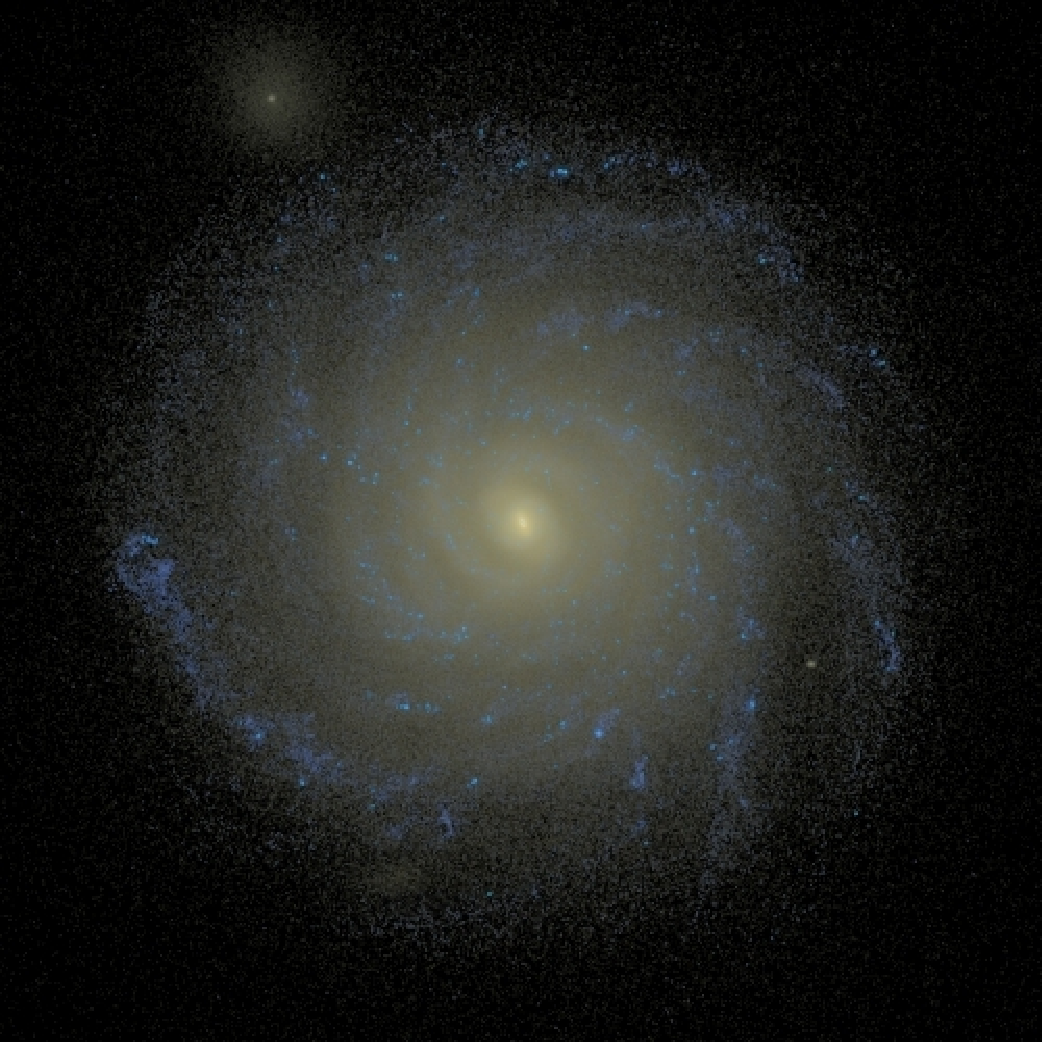
\includegraphics[width=\columnwidth]{Figures/boring}
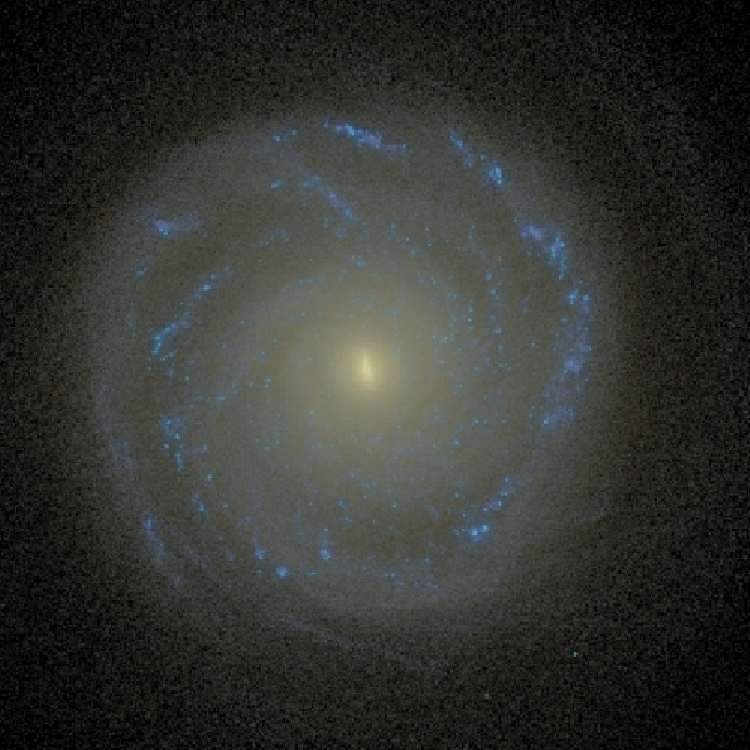
\includegraphics[width=\columnwidth]{Figures/exciting}
\caption{Synthetic SDSS $gri$ images of our two Milky Way-type galaxies, h277 (left) and h258 (right), created with \textsc{SUNRISE} \citep{Jonsson06}.
\label{fig:images}
}
\end{figure*}


\begin{figure*}
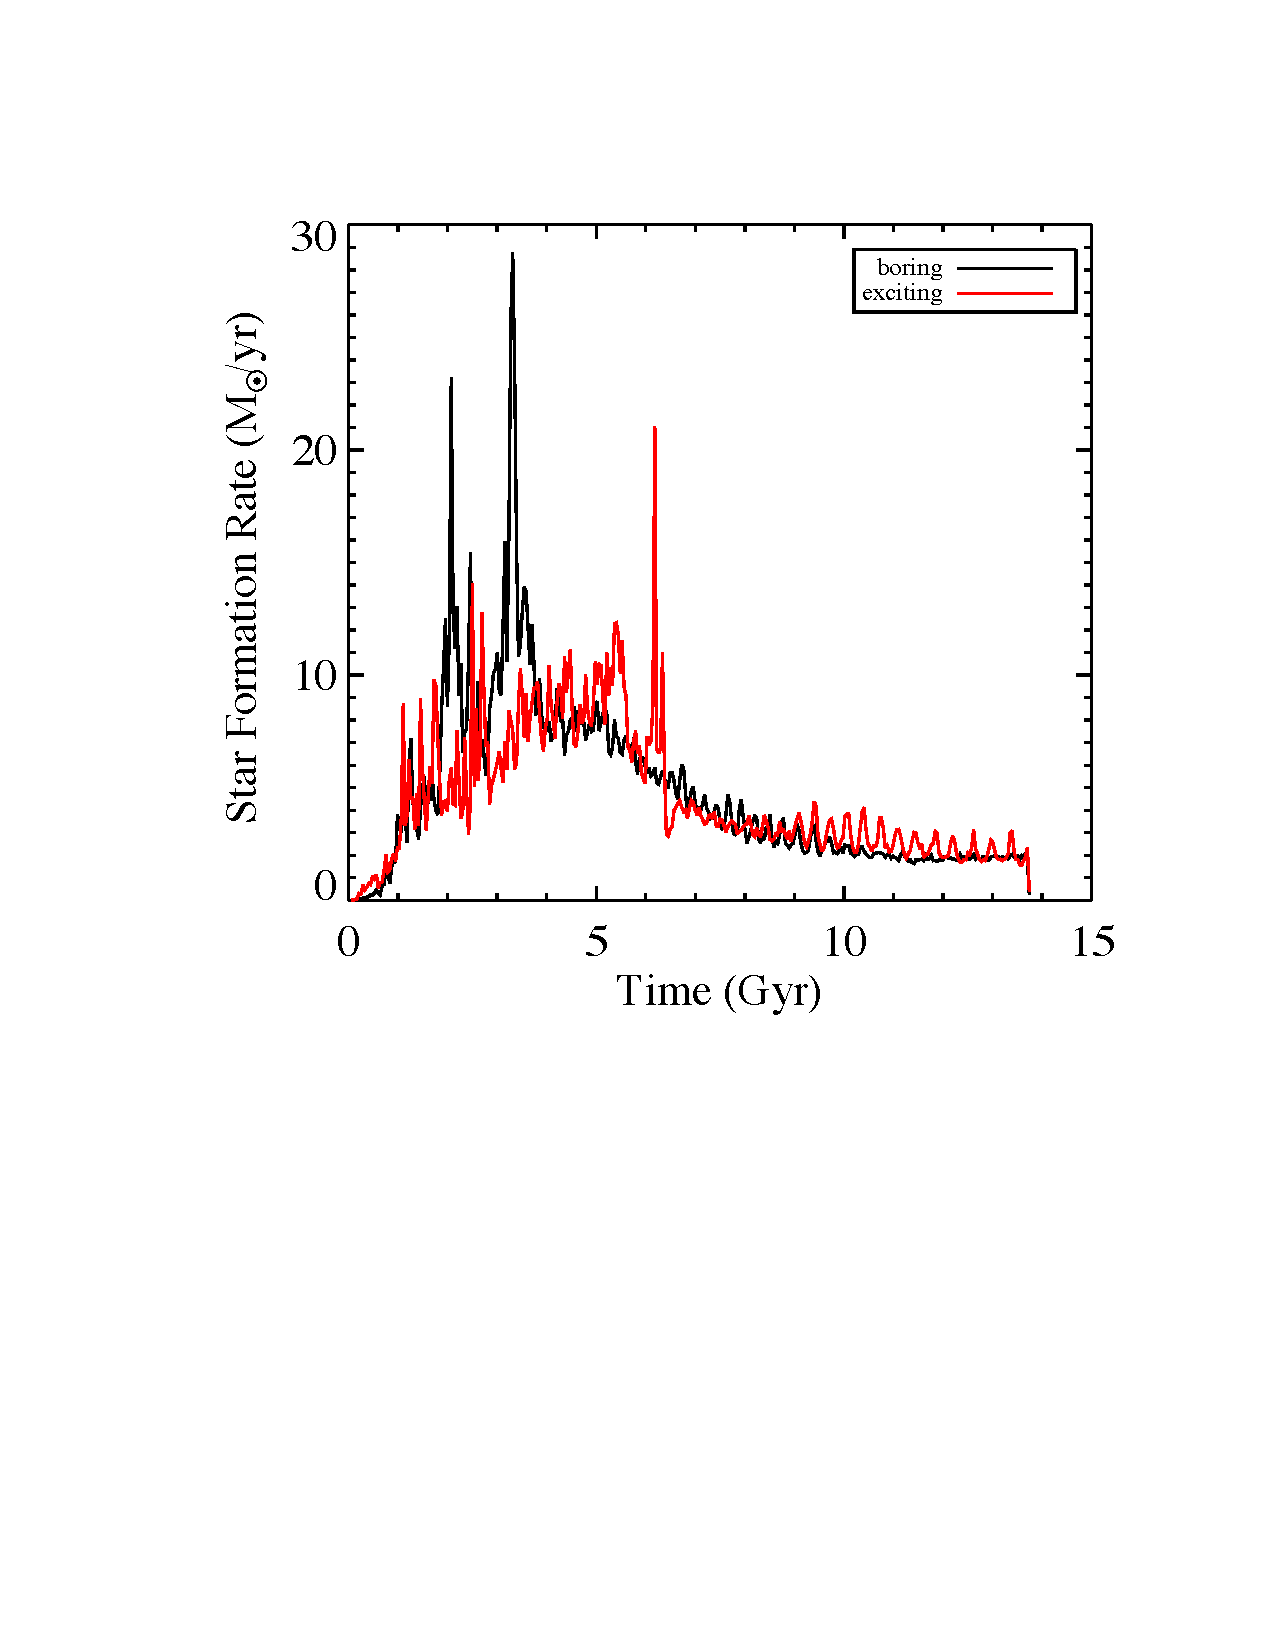
\includegraphics[width=\columnwidth]{Figures/sfh}
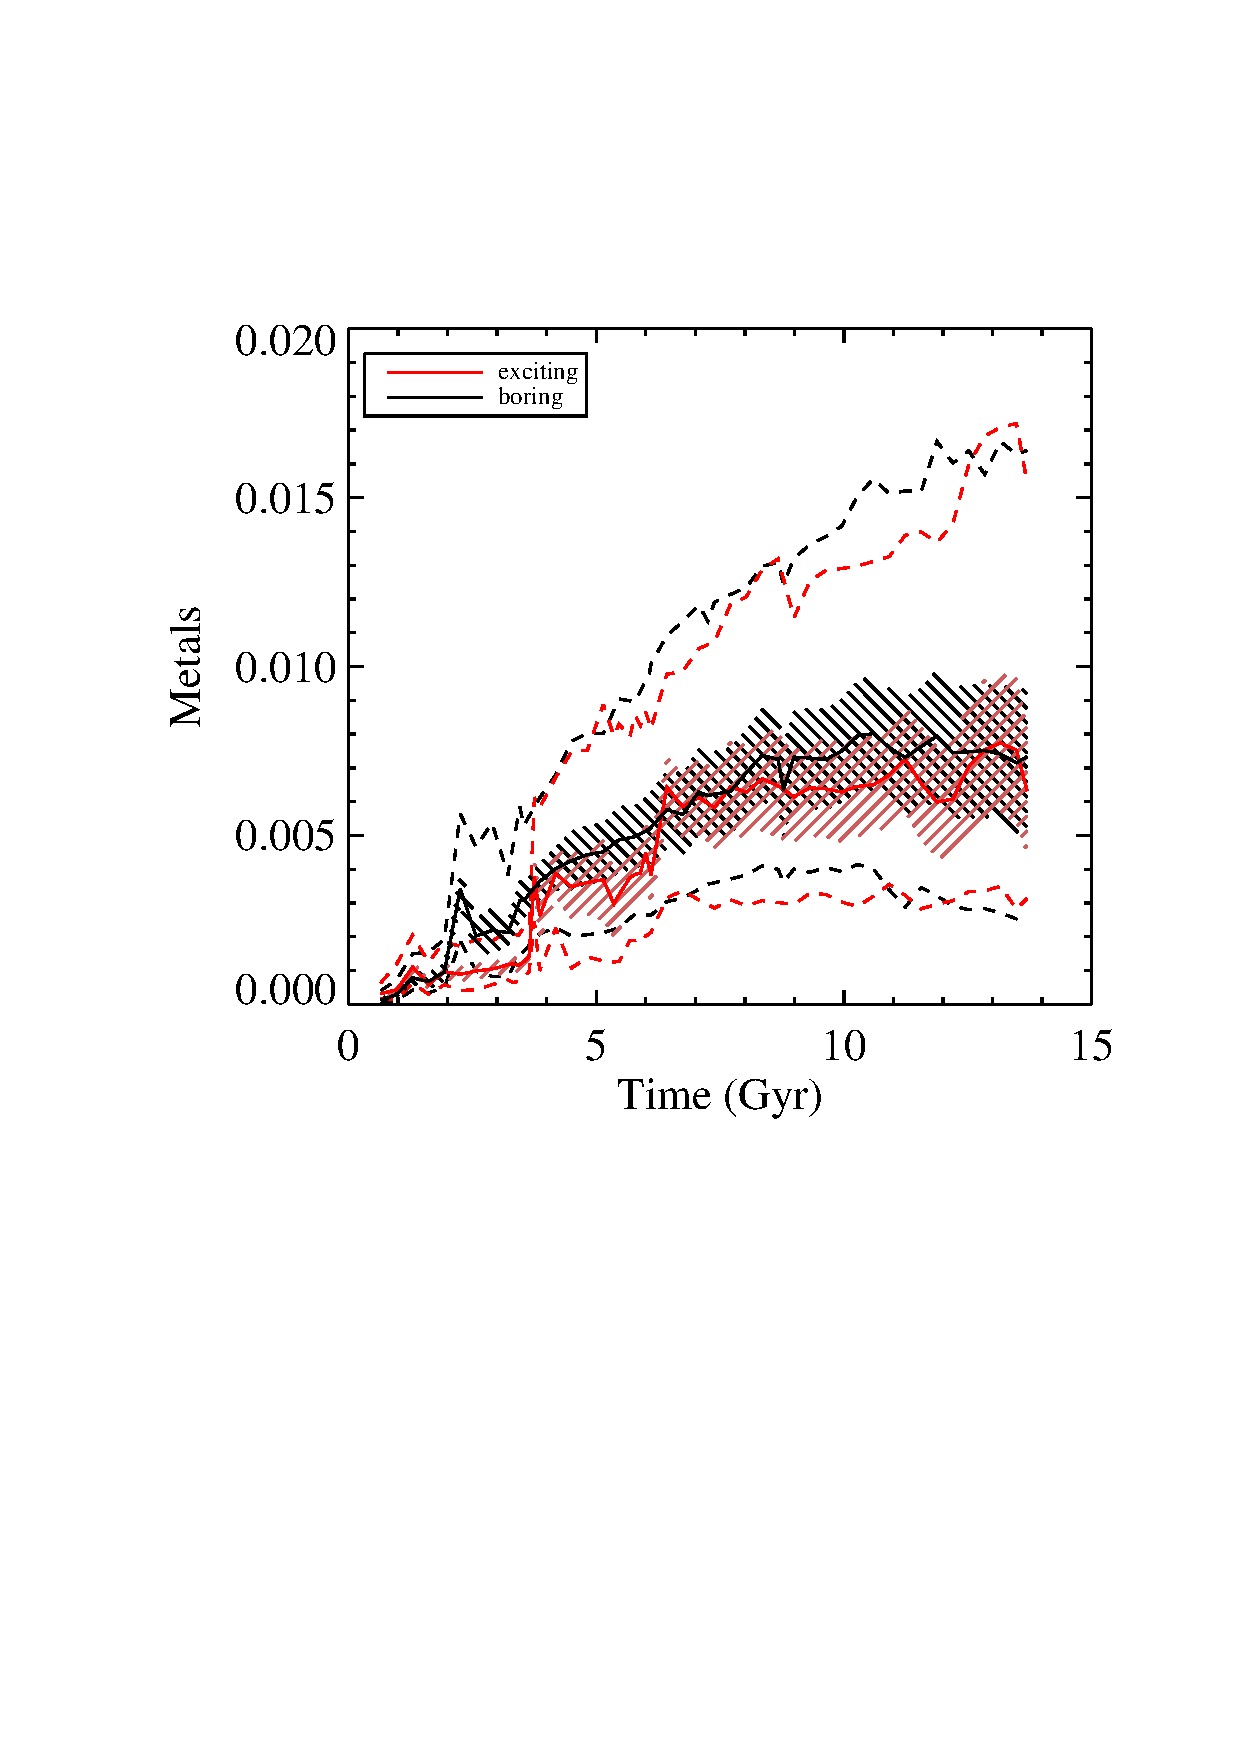
\includegraphics[width=\columnwidth]{Figures/zvst}
\caption{\label{fig:TwoGalaxies}\textbf{Star formation and metallicity versus time}:  \emph{Left panel}: Star formation history $\dot{M}_{*}$
  versus time.  Black corresponds to galaxy A (``boring'') and red to galaxy B (``exciting'').  
\emph{Right panel}: A plot of the  metallicity $Z$ of recently-formed stars versus time.  Solid red and black lines show
the mean metallicity; dotted lines correspond to  90\% of newly-born stars have lower metallicity,   or 10\% of
newly-born stars have greater metallicity.  When these two galaxies are $2-3\unit{Gyr}$ old, prior to the first major
merger of  near the peak of their
star-forming history, newly-born stars are created with significantly different metallicity.  Additionally, prior to the
second major merger of galaxy B at $\simeq 6\unit{Gyr}$, stars form in the ``exciting'' galaxy at a systematically lower
metallicity than in the ``boring'' counterpart.
}
\end{figure*}

\section{Detection-weighted compact binary formation}
\label{sec:model}

Our goal in this work is to estimate the \emph{ratio} of compact binaries that should be merging, at present, in the two
simulated galaxies described above.

To explore plausible binary detection scenarios, we adopt a parameterized formalism for binary evolution and event
detection in an individual galaxy, motivated by
the detailed studies of  \abbrvPSgrb{} and \abbrvPSellipticals; \jillianremark{this is first mention of PSG and PSE, define} similar approaches have been used by
\cite{2016arXiv160508783L} and others.


Binary evolution calculations suggest the binary compact object formation rate rate depends sensitively on the assumed metallicity, in conjunction
with other parameters \citep[see,\,e.g.][and references
  therein]{popsyn-LowMetallicityImpact-Chris2008,popsyn-LIGO-SFR-2008,gwastro-EventPopsynPaper-2016}.
% POINT: 
%   - final BH spin, mass can change number favored
%   - of course
Gravitational wave detectors are also far more sensitive to  massive compact binaries, which are  preferentially  formed in low metallicity
environments \citep{PSellipticals,popsyn-LowMetallicityImpact2c-StarTrackRevised-2014}.  As a result, low metallicity
environments can be overwhelmingly efficient factories for detectable black hole binaries
\citep{popsyn-LowMetallicityImpact2c-StarTrackRevised-2014,gwastro-EventPopsynPaper-2016}.  
%
For this reason, our estimates for compact binary coalescence rates must account for how often  different star-forming
conditions occur;  how often compact binaries that can coalesce now can derive from each environment; and how often LIGO will detect compact
binaries with different masses, all other things being equal.

\begin{widetext}
% POINT:  Model
To characterize how much more likely LIGO will detect coalescing binaries with different masses, we use a common and
naive estimate for the volume to which advanced LIGO is sensitive \citep[see,e.g.,][]{PSellipticals}:\footnote{For
  simplicity, in this calculation we neglect the effects of cosmology; strong field coalescence; and black hole spin;
  see \cite{popsyn-LowMetallicityImpact2c-StarTrackRevised-2014}, \cite{AstroPaper}, or \cite{RatesPaper} for more details.}
\begin{eqnarray}
V = \frac{4\pi}{3} [445 \unit{Mpc}]^3 \int p(m_1,m_2|Z) dm_1 dm_2 [ (\mc/1.2 M_\odot)^{5/6}]^3
\end{eqnarray}
where $\mc\equiv (m_1 m_2)^{3/5}/(m_1+m_2)^{1/5}$.   
This expression depends explicitly on an assumed and metallicity-dependent mass distribution for compact object
mergers, through the characteristic chirp mass $\mc_{*}(Z)\equiv [\int p(m_1,m_2|Z) dm_1 d,m_2 (\mc/1.2
  M_\odot)^{15/6}]^{5/16}$ .  We calibrate our metallicity-dependent mass distributions to metallicity-dependent binary
evolution calculations presented in \cite{popsyn-LowMetallicityImpact2-StarTrackRevised-2012} and
\cite{popsyn-LowMetallicityImpact2c-StarTrackRevised-2014}; see, e.g., their Table 1 and Figures 5-7.    For neutron
stars, we adopt a fiducial neutron star mass of $1.4 M_\odot$ at all metallicities.  For BH-NS binaries, we adopt a
highly simplified model: the black hole masses are uniformly \editremark{fixme?} drawn from $5 M_\odot$ to the maximum 
black hole mass $M_{max}(Z)$ allowed by
\emph{isolated} stellar evolution, as reported in prior work \citep[see,e.g.][and references
  therein]{gwastro-EventPopsynPaper-2016}.  In agreement with much more detailed prior work \cite{popsyn-LowMetallicityImpact2c-StarTrackRevised-2014}, this simplified model yields typical chirp masses for BH-NS binaries that
vary slightly as $Z/Z_\odot$ decreases, from a lower limit of $3 M_\odot$ near solar metallicity to an upper limit of
$4.3 M_\odot$ in low-metallicity environments.  Finally, for binary black holes, we assume  comparable-mass binaries
form ($m_1=m_2$), with the distribution of component masses chosen to be $\propto m_1^{-p}$ 
 between $3 M_\odot$ and $M_{max}(Z)$ and zero otherwise, adopting a fiducial exponent $p=2$; see, e.g.,
\cite{popsyn-LowMetallicityImpact2b-StarTrackRevised-2013}.    For binary black holes, this means  the
detection-weighted mass distribution [$\propto p(m_1,m_2)
\mc^{15/6}$] depends weakly on mass [$ p(m_1,m_2)
\mc^{15/6} \propto m_1^{-0.5} \delta(m_1-m_2)$.  In our simple model, the total  and chirp mass
distributions   are qualitatively consistent with detailed  binary evolution calculations \citep{popsyn-LowMetallicityImpact2b-StarTrackRevised-2013}. 

\end{widetext}

% POINT:  Model
To characterize the frequency of different star-forming conditions, we use our cosmological simulations of Milky Way-like galaxies, which provide each galaxy's star formation rate
$\dot{M}_*$ and star formation metallicity distribution $p(\log Z|t)$ over time.

% POINT: 
To characterize how often compact binaries form and coalesce, we use the ansatz adopted in \abbrvPSellipticals{} and
\abbrvPSgrb{}: for a star-forming parcel of mass $\Delta M$ the number of binaries born at time $0$ which
are coalescing now is $\lambda \Delta M dP/dt$, where $\lambda$ is an overall efficiency per unit mass and $P(<t|Z)$ is
a metallicity-dependent delay time distribution.\footnote{For simplicity, we assume the mass and delay time
  distributions are uncorrelated.  Figure A9 in \abbrvPSgrb{} shows this approximation, while not strictly true, is an
  excellent approximation for merging BH-BH binaries at solar metallicity.  }
    In this paper we are investigating the relative contribution of
different star-forming environments and galaxy evolutionary histories, not the overall normalization, so the overall scale of $\lambda$ is irrelevant.  
However, to account for the strong tendency of low-metallicity star-forming regions to produce many binary compact
objects, we adopt a power law
\begin{eqnarray}
\label{eq:LambdaVersusZModel}
\lambda(Z) &=& \lambda_o \text{min}[(Z/Z_\odot)^{-a}, F_{max}] 
\end{eqnarray}
with $a\in [0,3]$ and $F_{max}<10^3$
%$\lambda_o F_{max} < 3\times 10^{-4}/M_\odot$
 (see, e.g.\cite{popsyn-LIGO-SFR-2008}, \abbrvKBLowZa).  For the purposes of illustration, we adopt a  concrete scale
factor  $
\lambda_0 = 10^{-3}/M_\odot $,  a typical value suitable for neutron star compact binaries (see \abbrvPSgrb{}, \abbrvPSellipticals, and \abbrvKBLowZa).
%
For binaries containing neutron stars, for simplicity and without loss of generality we adopt the universal delay time distribution
%% Finally, we parameterize the delay time distribution by  either
%% \begin{eqnarray}
%% P_t(<t) &=& \begin{cases}
%% 0 & t<10 \unit{Myr} \\
%% (t/13\unit{Gyr})^{b}& t \in [10\unit{Myr},t_H]
%% \end{cases} 
%% \end{eqnarray}
%% with $b> 0$ or as the special case
\begin{eqnarray}
\frac{dP_t(<t)}{dt} =  \begin{cases}
0 & t<10 \unit{Myr} \\
\frac{1}{t \ln (13 \unit{Gyr}/10\unit{Myr})} & t \in [10\unit{Myr},13\unit{Gyr}]
\end{cases} 
\end{eqnarray}
\abbrvPSgrb{} and \abbrvPSellipticals{} show this distribution is reasonable approximations to compact binary delay
time distributions.\footnote{Simulations suggest the delay time distribution varies from model to model and with mass.
  These variations have less impact on our results than the evolving metallicity distribution of star forming gas.}
%
For suitable choices of parameter, our phenomenological response function is qualitatively consistent with the results of detailed simulations of binary
evolution  \citep{2010ApJ...715L.138B,popsyn-LowMetallicityImpact2c-StarTrackRevised-2014,popsyn-LowMetallicityImpact2b-StarTrackRevised-2013,popsyn-LowMetallicityImpact2-StarTrackRevised-2012}.


For binary black holes formed near solar metallicity, the delay time distribution can favor long delays between birth
and merger, as demonstrated in Figures 9 and 10 of \abbrvPSellipticals{}.  [Figure 2 of  \cite{2016arXiv160508783L} is
  an extreme example of this well-known trend.]  In practice, however, binary black holes produced near solar
metallicity correspond to a relatively small proportion of the overall population; we therefore neglect this
effect\footnote{may want to change}.


% POINT: Net effect
Therefore, up to an irrelevant overall scale factor, the  present-day detection-weighted coalescence rate $r_D$  of binary compact objects formed by within two similar
galaxies  can be calculated via
\begin{eqnarray}
 r_D \propto  \int d\log Z  \int _{13 \unit{Gyr}}^0dt  V(Z) \lambda(Z) \frac{dP}{dt}(t) \dot{M} p(\log Z|t)
\end{eqnarray}


\section{Formation rate for binary black holes}
\label{sec:results:BBH}



\section{Implications for transient multimessenger astronomy}

Our calculations suggest that because of the often-long delays between formation and merger, combined with the
propensity of low-metallicity gas to play an exceptionally significant role, unusually detailed information about each host galaxy could be required to realize the full
potential of  associations between gravitational wave sources and their candidate host galaxies.
%
Fortunately,  with the advent of
IFUs and position-resolved spectroscopy, observers can now probe the star formation history and metallicity of
individual gas packets at different points in a galaxy.  
%
These highly-detailed probes will be essential tools to develop a comprehensive model of the galaxy's merger and
chemical evolution history.    

Even when electromagnetic counterparts are available, the long delay times between coalescence and merger \jillianremark{(hold on are coalescence and mergers not the same thing?  does coalescence represent the beginning of the inspiral?  hmmm)} limit
the prospects of detailed electromagnetic followup of individual event. 
The metallicity of stars and gas adjacent to a specific merger event provides
few direct, unambiguous clues to a compact binary merger's progenitors.  
On the one hand, compact binaries are kicked by supernovae, moving substantially away from their birth position
%  2014arXiv1407.3796S : implications for nucleosynthesis
\cite{2013ApJ...776...18F,2014ARAA..52...43B}. 
On the other hand, particularly during the epoch of galaxy formation, galaxies are well-mixed: stars and adjacent gas generally do not have
similar chemical composition.  
% POINT: Host tracer gas --we are optimistically assuming the metallicity 
%  can be measured.  A seperate question is whether you can measure Z in the local environment at all.
These mixing effects have been previously recognized as an obstacle to interpreting transient event spectra.  For
example,   \cite{2010MNRAS.402.1523P} previously demonstrated that absorbing gas neighboring transient events (there, long GRBs)
would generally have high metallicity, even for low-metallicity progenitors.   
%
\citet{2010MNRAS.402.1523P} have previously used hydrodynamical simulations to demonstrate that observed ambient
metallicities (there, using damped Lyman $\alpha$ absorbers in the host) do not tightly constrain the metallicity
distribution of the progenitor; see, e.g., their Fig 3.
%


% POINT: 
Despite the challenges involved in obtaining sufficient statistics, possibly requiring third-generation instruments to
obtain sufficiently many associations, past experience suggests  host galaxy associations
will provide unique clues into the formation mechanism of compact binaries.
% 
Each host galaxy associates a merger to a unique star formation history and metallicity distribution.
With many events, these associations can potentially determine the ``response function'' for compact binaries: how often star forming gas of a given metallicity evolves into
merging compact binaries.    
%
For example, in several cases the metallicity of gas neighboring a long GRB (\citet{ 2008AJ....135.1136M}; \citet{2010AJ....140.1557L}
\editremark{links}), short GRB (\editremark{XXX}), or SN has been directly measured.
%
The precise host offset can be compared to the distribution of light and star formation  \citep{2010ApJ...708....9F}.
%
Finally,  on a host-by-host basis, the delay time between birth and merger has been constrained for long GRBs (\editremark{XXX}), short GRBs \citep{2010ApJ...725.1202L}, and
  SN Ia \citep{2011MNRAS.412.1508M}.  
%
The future of gravitational wave host galaxy associations is bright.




% POINT: Observations provide sample of extragalactic  binaries at merger, and  host galaxies.  Possible to mine large archive of events
% to deduce correlations

%% %
%% Highly atypical formation scenarios seemingly should produce events in or near atypical hosts.  
%% % POINT: Introduce *idea* of comparison: refs for mass-metallicity relation
%% For example, in the local universe galaxies lie along mass-metallicity  (\cite{2004ApJ...613..898T}; see also
%% \cite{sfr-ZEvolution-ByGalaxy-Panter2008})
%% or mass-metallicity-star formation rate  correlations (e.g., \cite{2010MNRAS.408.2115M}).
%% % POINT: Evolution tricky
%% [The change in these correlations with redshift is still being investigated; see, e.g., \editremark{citation: Panter;
%%     Mannucci; }, \cite{2011ApJ...739....1L} and references therein.]
%% % POINT: previous studies
%% Based on these correlations, both short  and long GRBs seem to arise from
%% relatively typical hosts at their redshift; see, e.g., \cite{grb-short-Hosts-Berger2008} and \cite{grb-long-HostMetallicityVsTrend-Mannucci2010}.





\section{Conclusions}

We present a model for binary black hole \jillianremark {and other binary compact object formation?} based on models of binary formation and properties over cosmic time.  We fold these models with star formation histories and metallicity distributions taken from state of the art cosmological simulations of Milky Way-like galaxies.  We demonstrate that galaxies which appear similar at $z = 0$ but have differing merger histories will have different rates of BBH mergers detectable by LIGO.  \jillianremark{sentence detailing the specifics of this prediction, once we know what it is.}   

One result of our conclusions is that we can learn about the past assembly history of a galaxy from its LIGO event rate, \jillianremark{ that's really cool.  }  Also we can use resolved star formation histories of nearby galaxies {\bf (citations)} to predict likelihoods for LIGO events.  \jillianremark { what else}\\


* BBH properties far from apparent.  No surprise: delays can be long \cite{PSellipticals,popsyn-LowMetallicityImpact2b-StarTrackRevised-2013,gwastro-EventPopsynPaper-2016}, particularly because formation in low Z favored,
so system changes significantly from assembly conditions

* EM counterpart properties: delay times are shorter, so more of a surprise that formation scenario matters.  However,
BH properties depend on $Z$, which can influence the mass and spin of BHs that produce EM counterparts.



* Detailed analysis of one host galaxy presented in this work is complementary to the population-based approach used in
\cite{2016arXiv160508783L}, which favored formation in a wide range of galaxies and event times.   % that analysis also
                                % used a poor input from BSE, about the coalescence delay

Biases towards low-metallicity star formation have been extensively studied in the context of long GRBs and their host galaxies.
%
For example, \cite{2009ApJ...702..377K} demonstrated that a sufficiently strong bias towards low-metallicity star formation would predict
most  events in the local universe occur low-mass and dwarf galaxies.
%<
For less extreme metallicity biases, subsequent calculations by  \citet{2011MNRAS.417..567N} demonstrated that the



% POINT: Future directions

\begin{acknowledgements}
ROS acknowledges support from NSF award AST-1412449, via subcontract from the University of Wisconsin-Milwaukee.
%
JB acknowledges generous support  from the Helen Gurley Brown Trust.
\end{acknowledgements}

\appendix






\bibliography{bhmetals}
\end{document}
